Договоримся о способе <<одномерной>> нумерации неизвестных.
Будем нумеровать неизвестные по строкам, то есть вдоль оси $x$.
Имеем следующую формулу для обобщенного индекса.
\[ m = j (N_x + 1) + i \]
Индексы изменяются в следующих границах
\[ 0 \leq i \leq N_x \]
\[ 0 \leq j \leq N_y \]
и тогда
\[ 0 \leq m < (N_x + 1) (N_y + 1) \]

% done
\subsection{Запись для внутренних точек}
Перепишем уравнения для $i = \overline{1,N_x-1}$ и $j = \overline{1,N_y-1}$ с использовнием нового индекса.
\begin{multline*}
    - \left[
    h_y k_1(x_{i+1/2},y_{j}) \frac{v_{i+1,j} - v_{i,j}}{h_x} - h_y k_1(x_{i-1/2},y_{j}) \frac{v_{i,j} - v_{i-1,j}}{h_x} + \right. \\
    \left. +
    h_x k_2(x_{i},y_{j+1/2}) \frac{v_{i,j+1} - v_{i,j}}{h_y} - h_x k_2(x_{i},y_{j-1/2}) \frac{v_{i,j} - v_{i,j-1}}{h_y}
    \right] =
    h_x h_y f_{i,j}
\end{multline*}
\[
\begin{split}
    &-\frac{h_x}{h_y} k_2(x_{i},y_{j-1/2}) v_{i,j-1} - \frac{h_y}{h_x} k_1(x_{i-1/2},y_{j}) v_{i-1,j} + \\
    &+\left[ \frac{h_x}{h_y} k_2(x_{i},y_{j-1/2}) + \frac{h_y}{h_x} k_1(x_{i-1/2},y_{j}) + \frac{h_y}{h_x} k_1(x_{i+1/2},y_{j}) + \frac{h_x}{h_y} k_2(x_{i},y_{j+1/2}) \right] v_{i,j} - \\
    &-\frac{h_y}{h_x} k_1(x_{i+1/2},y_{j}) v_{i+1,j} - \frac{h_x}{h_y} k_2(x_{i},y_{j+1/2}) v_{i,j+1} = h_x h_y f_{i,j}
\end{split}
\]
Введем новые обозначения
\[ a_m w_{m - L} + b_m w_{m - 1} + c_m w_m + d_m w_{m + 1} + e_m w_{m + L} = g_m \]
Тогда получаем формулы для коэффициентов системы
\[ a_m = -\frac{h_x}{h_y} k_2(x_{i},y_{j-1/2}) \]
\[ b_m = -\frac{h_y}{h_x} k_1(x_{i-1/2},y_{j}) \]
\[ c_m = \frac{h_x}{h_y} k_2(x_{i},y_{j-1/2}) + \frac{h_y}{h_x} k_1(x_{i-1/2},y_{j}) + \frac{h_y}{h_x} k_1(x_{i+1/2},y_{j}) + \frac{h_x}{h_y} k_2(x_{i},y_{j+1/2}) \]
\[ d_m = -\frac{h_y}{h_x} k_1(x_{i+1/2},y_{j}) \]
\[ e_m = -\frac{h_x}{h_y} k_2(x_{i},y_{j+1/2}) \]
\[ g_m = h_x h_y f_{i,j} \]
% \begin{figure}[H]
%     \centering
%     \includegraphics[width=0.5\textwidth]{img/inner-crop.pdf}
% \end{figure}

\subsection{Запись для левой границы}
Перепишем уравнения для $i = 0$ и $j = \overline{1,N_y-1}$ с использовнием нового индекса.
\begin{multline*}
    - \left[
    h_y k_1(x_{1/2},y_{j}) \frac{v_{1,j} - v_{0,j}}{h_x} - h_y \left( \chi_1 v_{0,j} - g_1(y_{j}) \right) + \right. \\
    \left. +
    \frac{h_x}{2} k_2(x_{0},y_{j+1/2}) \frac{v_{0,j+1} - v_{0,j}}{h_y} - \frac{h_x}{2} k_2(x_{0},y_{j-1/2}) \frac{v_{0,j} - v_{0,j-1}}{h_y}
    \right] =
    \frac{h_x}{2} h_y f_{0,j}
\end{multline*}
\[
\begin{split}
    &-\frac{h_x}{2 h_y} k_2(x_{0},y_{j-1/2}) v_{0,j-1} +\\
    &+\left[ \frac{h_x}{2 h_y} k_2(x_{0},y_{j-1/2}) + \frac{h_y}{h_x} k_1(x_{1/2},y_{j}) + \frac{h_x}{2 h_y} k_2(x_{0},y_{j+1/2}) + h_y \chi_1 \right] v_{0.j} - \\
    &-\frac{h_y}{h_x} k_1(x_{1/2},y_{j}) v_{1,j} - \frac{h_x}{2 h_y} k_2(x_{0},y_{j+1/2}) v_{0,j+1} = \frac{h_x}{2} h_y f_{0,j} + h_y g_1(y_j)
\end{split}
\]
\[ a_m w_{m - L} + c_m w_m + d_m w_{m + 1} + e_m w_{m + L} = g_m \]
Тогда получаем формулы для коэффициентов системы
\[ a_m = -\frac{h_x}{2 h_y} k_2(x_{0},y_{j-1/2}) \]
\[ c_m = \frac{h_x}{2 h_y} k_2(x_{0},y_{j-1/2}) + \frac{h_y}{h_x} k_1(x_{1/2},y_{j}) + \frac{h_x}{2 h_y} k_2(x_{0},y_{j+1/2}) + h_y \chi_1 \]
\[ d_m = -\frac{h_y}{h_x} k_1(x_{1/2},y_{j}) \]
\[ e_m = -\frac{h_x}{2 h_y} k_2(x_{0},y_{j+1/2}) \]
\[ g_m = \frac{h_x}{2} h_y f_{0,j} + h_y g_1(y_j) \]
% \begin{figure}[H]
%     \centering
%     \includegraphics[width=0.5\textwidth]{img/left-crop.pdf}
% \end{figure}

\subsection{Запись для правой границы}
Перепишем уравнения для $i = N_x$ и $j = \overline{1,N_y-1}$ с использовнием нового индекса.
\[ v_{N_x,j} = g_2(y_j) \]
\[ c_m w_m = g_m \]
Тогда получаем формулы для коэффициентов системы
\[ c_m = 1 \]
\[ g_m = g_2(y_j) \]
% \begin{figure}[H]
%     \centering
%     \includegraphics[width=0.5\textwidth]{img/right-crop.pdf}
% \end{figure}

\subsection{Запись для нижней границы}
Перепишем уравнения для $i = \overline{1,N_x-1}$ и $j = 0$ с использовнием нового индекса.
\begin{multline*}
    - \left[
    \frac{h_y}{2} k_1(x_{i+1/2},y_0) \frac{v_{i+1,0} - v_{i,0}}{h_x} - \frac{h_y}{2} k_1(x_{i-1/2},y_0) \frac{v_{i,0} - v_{i-1,0}}{h_x} + \right. \\
    \left. +
    h_x k_2(x_i,y_{1/2}) \frac{v_{i,1} - v_{i,0}}{h_y} - h_x \left( \chi_3 v_{i,0} - g_3(x_i) \right)
    \right] =
    h_x \frac{h_y}{2} f_{i,0}
\end{multline*}
\[
\begin{split}
    &-\frac{h_y}{2 h_x} k_1(x_{i-1/2},y_0) v_{i-1,0} +\\
    &+\left[ \frac{h_y}{2 h_x} k_1(x_{i-1/2},y_0) + \frac{h_y}{2 h_x} k_1(x_{i+1/2},y_0) + \frac{h_x}{h_y} k_2(x_i,y_{1/2}) + h_x \chi_3 \right] v_{i.0} - \\
    &- \frac{h_y}{2 h_x} k_1(x_{i+1/2},y_0) v_{i+1,0} - \frac{h_x}{h_y} k_2(x_i,y_{1/2}) v_{i,1} = h_x \frac{h_y}{2} f_{i,0} + h_x g_3(x_i)
\end{split}
\]
\[ b_m w_{m - 1} + c_m w_m + d_m w_{m + 1} + e_m w_{m + L} = g_m \]
Тогда получаем формулы для коэффициентов системы
\[ b_m = -\frac{h_y}{2 h_x} k_1(x_{i-1/2},y_0) \]
\[ c_m = \frac{h_y}{2 h_x} k_1(x_{i-1/2},y_0) + \frac{h_y}{2 h_x} k_1(x_{i+1/2},y_0) + \frac{h_x}{h_y} k_2(x_i,y_{1/2}) + h_x \chi_3 \]
\[ d_m = -\frac{h_y}{2 h_x} k_1(x_{i+1/2},y_0) \]
\[ e_m = -\frac{h_x}{h_y} k_2(x_i,y_{1/2}) \]
\[ g_m = h_x \frac{h_y}{2} f_{i,0} + h_x g_3(x_i) \]
% \begin{figure}[H]
%     \centering
%     \includegraphics[width=0.5\textwidth]{img/bottom-crop.pdf}
% \end{figure}

\subsection{Запись для верхней границы}
Перепишем уравнения для $i = \overline{1,N_x-1}$ и $j = N_y$ с использовнием нового индекса.
\begin{multline*}
    - \left[
    \frac{h_y}{2} k_1(x_{i+1/2},y_{N_y}) \frac{v_{i+1,N_y} - v_{i,N_y}}{h_x} - \frac{h_y}{2} k_1(x_{i-1/2},y_{N_y}) \frac{v_{i,N_y} - v_{i-1,N_y}}{h_x} + \right. \\
    \left. +
    h_x \left( - \chi_4 v_{i,N_y} + g_4(x_i) \right) - h_x k_2(x_i,y_{N_y-1/2}) \frac{v_{i,N_y} - v_{i,N_y-1}}{h_y}
    \right] =
    h_x \frac{h_y}{2} f_{i,N_y}
\end{multline*}
\[
\begin{split}
    &-\frac{h_x}{h_y} k_2(x_i,y_{N_y-1/2}) v_{i,N_y-1} - \frac{h_y}{2 h_x} k_1(x_{i-1/2},y_{N_y}) v_{i-1,N_y} +\\
    &+\left[ \frac{h_x}{h_y} k_2(x_i,y_{N_y-1/2}) + \frac{h_y}{2 h_x} k_1(x_{i-1/2},y_{N_y}) + \frac{h_y}{2 h_x} k_1(x_{i+1/2},y_{N_y}) + h_x \chi_4 \right] v_{i,N_y} - \\
    &-\frac{h_y}{2 h_x} k_1(x_{i+1/2},y_{N_y}) v_{i+1,N_y} = h_x \frac{h_y}{2} f_{i,N_y} + h_x g_4(x_i)
\end{split}
\]
\[ a_m w_{m - L} + b_m w_{m - 1} + c_m w_m + d_m w_{m + 1} = g_m \]
Тогда получаем формулы для коэффициентов системы
\[ a_m = -\frac{h_x}{h_y} k_2(x_i,y_{N_y-1/2}) \]
\[ b_m = -\frac{h_y}{2 h_x} k_1(x_{i-1/2},y_{N_y}) \]
\[ c_m = \frac{h_x}{h_y} k_2(x_i,y_{N_y-1/2}) + \frac{h_y}{2 h_x} k_1(x_{i-1/2},y_{N_y}) + \frac{h_y}{2 h_x} k_1(x_{i+1/2},y_{N_y}) + h_x \chi_4 \]
\[ d_m = -\frac{h_y}{2 h_x} k_1(x_{i+1/2},y_{N_y}) \]
\[ g_m = h_x \frac{h_y}{2} f_{i,N_y} + h_x g_4(x_i) \]
% \begin{figure}[H]
%     \centering
%     \includegraphics[width=0.5\textwidth]{img/top-crop.pdf}
% \end{figure}

\subsection{Запись для левой нижней граничной точки}
Перепишем уравнения для $i = 0$ и $j = 0$ с использовнием нового индекса.
\begin{multline*}
    - \left[
    \frac{h_y}{2} k_1(x_{1/2},y_{0}) \frac{v_{1,0} - v_{0,0}}{h_x} - \frac{h_y}{2} \left( \chi_1 v_{0,0} - g_1(y_{0}) \right) + \right. \\
    \left. +
    \frac{h_x}{2} k_2(x_{0},y_{1/2}) \frac{v_{0,1} - v_{0,0}}{h_y} - \frac{h_x}{2} \left( \chi_3 v_{0,0} - g_3(x_{0}) \right)
    \right] =
    \frac{h_x}{2} \frac{h_y}{2} f_{0,0}
\end{multline*}
\[
\begin{split}
    &\left[ \frac{h_y}{2 h_x} k_1(x_{1/2},y_{0}) + \frac{h_x}{2 h_y} k_2(x_{0},y_{1/2}) + \frac{h_y}{2} \chi_1 + \frac{h_x}{2} \chi_3 \right] v_{0,0} - \\
    &-\frac{h_y}{2 h_x} k_1(x_{1/2},y_{0}) v_{1,0} - \frac{h_x}{2 h_y} k_2(x_{0},y_{1/2}) v_{0,1} = \frac{h_x}{2} \frac{h_y}{2} f_{0,0} + \frac{h_y}{2} g_1(y_0) + \frac{h_x}{2} g_3(x_0)
\end{split}
\]
\[ c_m w_m + d_m w_{m + 1} + e_m w_{m + L} = g_m \]
Тогда получаем формулы для коэффициентов системы
\[ c_m = \frac{h_y}{2 h_x} k_1(x_{1/2},y_{0}) + \frac{h_x}{2 h_y} k_2(x_{0},y_{1/2}) + \frac{h_y}{2} \chi_1 + \frac{h_x}{2} \chi_3 \]
\[ d_m = -\frac{h_y}{2 h_x} k_1(x_{1/2},y_{0}) \]
\[ e_m = -\frac{h_x}{2 h_y} k_2(x_{0},y_{1/2}) \]
\[ g_m = \frac{h_x}{2} \frac{h_y}{2} f_{0,0} + \frac{h_y}{2} g_1(y_0) + \frac{h_x}{2} g_3(x_0) \]
% \begin{figure}[H]
%     \centering
%     \includegraphics[width=0.5\textwidth]{img/left-bottom-crop.pdf}
% \end{figure}

\subsection{Запись для правой нижней граничной точки}
Перепишем уравнения для $i = N_x$ и $j = 0$ с использовнием нового индекса.
\[ v_{N_x,0} = g_2(y_0) \]
\[ c_m w_m = g_m \]
Тогда получаем формулы для коэффициентов системы
\[ c_m = 1 \]
\[ g_m = g_2(y_0) \]
% \begin{figure}[H]
%     \centering
%     \includegraphics[width=0.5\textwidth]{img/right-bottom-crop.pdf}
% \end{figure}

\subsection{Запись для правой верхней граничной точки}
Перепишем уравнения для $i = N_x$ и $j = N_y$ с использовнием нового индекса.
\[ v_{N_x,N_y} = g_2(y_{N_y}) \]
\[ c_m w_m = g_m \]
Тогда получаем формулы для коэффициентов системы
\[ c_m = 1 \]
\[ g_m = g_2(y_{N_y}) \]
% \begin{figure}[H]
%     \centering
%     \includegraphics[width=0.5\textwidth]{img/right-top-crop.pdf}
% \end{figure}

\subsection{Запись для левой верхней граничной точки}
Перепишем уравнения для $i = 0$ и $j = N_y$ с использовнием нового индекса.
\begin{multline*}
  - \left[
  \frac{h_y}{2} k_1(x_{1/2},y_{N_y}) \frac{v_{1,N_y} - v_{0,N_y}}{h_x} - \frac{h_y}{2} \left( \chi_1 v_{0,N_y} - g_1(y_{N_y}) \right) + \right. \\
  \left. +
  \frac{h_x}{2} \left( - \chi_4 v_{0,N_y} + g_4(x_0) \right) - \frac{h_x}{2} k_2(x_{0},y_{N_y-1/2}) \frac{v_{0,N_y} - v_{0,N_y-1}}{h_y}
  \right] =
  \frac{h_x}{2} \frac{h_y}{2} f_{0,N_y}
\end{multline*}
\[
\begin{split}
    &-\frac{h_x}{2 h_y} k_2(x_{0},y_{N_y-1/2}) v_{0,N_y-1} +\\
    &+\left[ \frac{h_x}{2 h_y} k_2(x_{0},y_{N_y-1/2}) + \frac{h_y}{2 h_x} k_1(x_{1/2},y_{N_y}) + \frac{h_y}{2} \chi_1 + \frac{h_x}{2} \chi_4 \right] v_{0,N_y} - \\
    &-\frac{h_y}{2 h_x} k_1(x_{1/2},y_{N_y}) v_{1,N_y} = \frac{h_x}{2} \frac{h_y}{2} f_{0,N_y} + \frac{h_y}{2} g_1(y_{N_y}) + \frac{h_x}{2} g_4(x_0)
\end{split}
\]
\[ a_m w_{m - L} + c_m w_m + d_m w_{m + 1} = g_m \]
Тогда получаем формулы для коэффициентов системы
\[ a_m = -\frac{h_x}{2 h_y} k_2(x_{0},y_{N_y-1/2}) \]
\[ c_m = \frac{h_x}{2 h_y} k_2(x_{0},y_{N_y-1/2}) + \frac{h_y}{2 h_x} k_1(x_{1/2},y_{N_y}) + \frac{h_y}{2} \chi_1 + \frac{h_x}{2} \chi_4 \]
\[ d_m = -\frac{h_y}{2 h_x} k_1(x_{1/2},y_{N_y}) \]
\[ g_m = \frac{h_x}{2} \frac{h_y}{2} f_{0,N_y} + \frac{h_y}{2} g_1(y_{N_y}) + \frac{h_x}{2} g_4(x_0) \]
% \begin{figure}[H]
%     \centering
%     \includegraphics[width=0.5\textwidth]{img/left-top-crop.pdf}
% \end{figure}

Удалим лишние элементы и получим систему с симметричной матрицей.
% \begin{figure}[H]
%     \centering
%     \includegraphics[width=0.5\textwidth]{img/extra-cells-crop.pdf}
% \end{figure}
Такую систему в соотвествии с вариантом работы будем решать методом сопряженных градиентов.

\subsection{Хранение матрицы системы}
При инициализации системы матрица хранится в координатном виде (\textbf{COO}rdinate format),
так как это кардинально упрощает добавление новых элементов.
% \begin{figure}[H]
%     \centering
%     \fbox{ 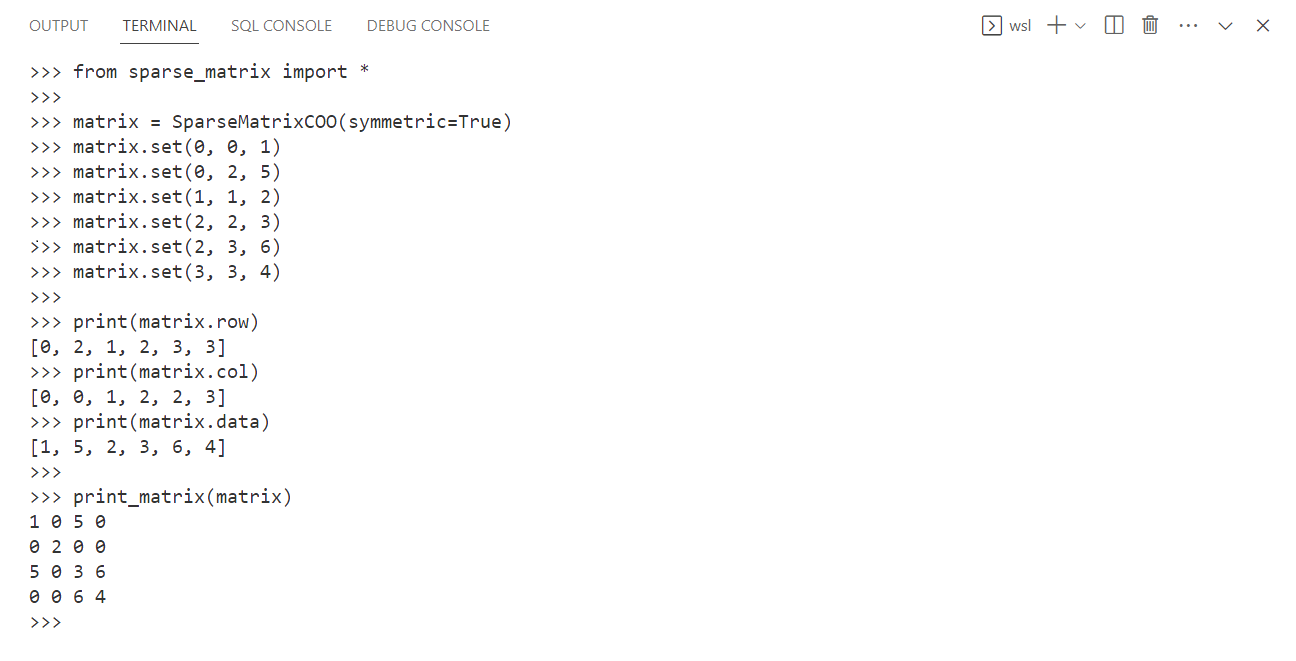
\includegraphics[width=0.95\textwidth]{img/sparse1.pdf} }
%     \caption{Инициализация матрицы}
% \end{figure}
После инициализации матрица переводится в сжатый разреженный строчный вид (\textbf{C}ompressed \textbf{S}parse \textbf{R}ow format),
и дальше сохраняет этот вид при всех последующих операциях с ней (при этом матрица становится неизменяемой).
% \begin{figure}[H]
%     \centering
%     \fbox{ 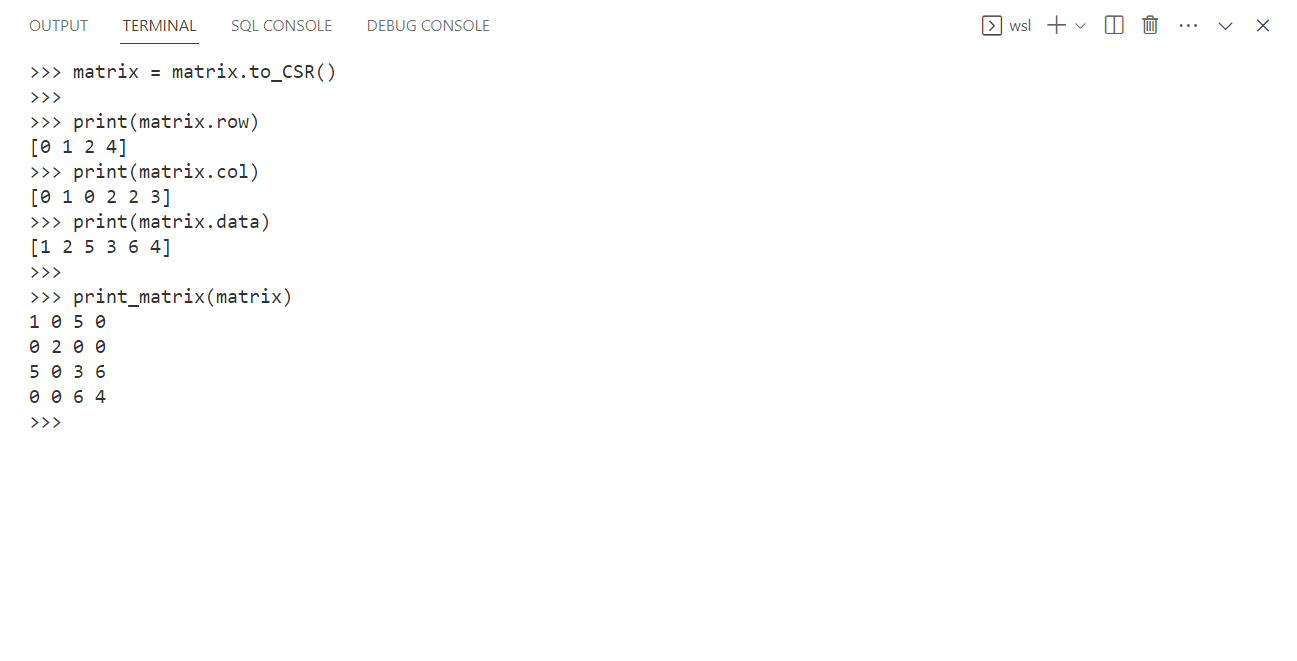
\includegraphics[width=0.95\textwidth]{img/sparse2.pdf} }
%     \caption{Перевод матрицы в новый вид}
% \end{figure}